\documentclass[border=10pt]{standalone}
\usepackage[european]{circuitikz}
\begin{document}
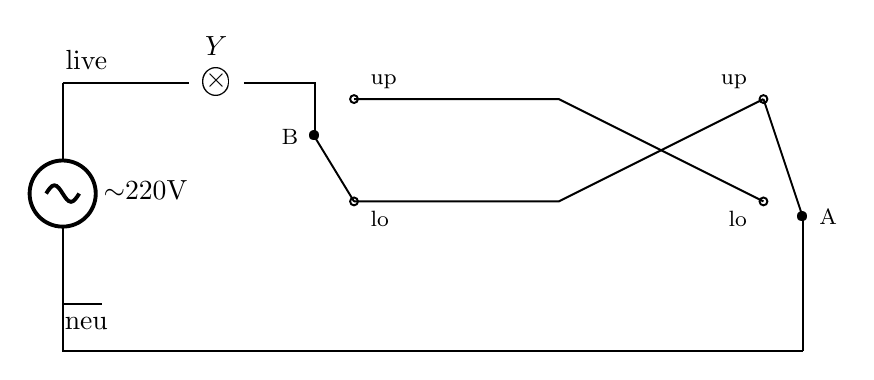
\begin{tikzpicture}[line width=0.7pt, font=\normalsize]

% 图 7.05 两处控制照明灯（习题 7.15）——照课程站 net-7-05 拓扑：
%   左侧：~220 V 正弦源，上端子 live、下端子 neu
%   live → 灯 Y(⊗) → bcom（B 的公共刀）；neu → A 的公共刀（ acom）
%   两条水平联络线在 A、B 之间：上线 live 侧↔live 侧？不——联络线连的是
%   A、B 的**触点**：B 的上触点(bup)与 A 的上触点(aup)一条线，B 的下触点
%   (blo)与 A 的下触点(alo)一条线（「上↔上、下↔下」为图库注释口径）。
%   刀位：B 向下（pos=2）、A 向上（pos=1）。
%   判据：灯必须 ⊗、电源必须正弦；两条联络线都要真的画出来。

% ── 电源（正弦）与上端子 ──
\draw (0,3.4) to[sinusoidal voltage source, l=$\sim$220V] (0,0.6);
\draw (0,3.4) -- (0.5,3.4);
\node[anchor=south] at (0.3,3.45) {live};
\draw (0,0.6) -- (0.5,0.6);
\node[anchor=north] at (0.3,0.55) {neu};
% 底部回线：neu → A 公共端（闭合回路）
\draw (0,0.6) -- (0,0.0) -- (9.4,0.0);

% ── 灯 Y（⊗）在 live 上 ──
\draw (0.5,3.4) -- (1.6,3.4);
\node at (1.95,3.4) {\textcircled{$\times$}};
\draw (2.3,3.4) -- (3.2,3.4) -- (3.2,2.72);
\node[anchor=south] at (1.95,3.62) {$Y$};

% ── B 开关（x=3.2）：公共刀 bcom 从灯右侧上来；触点 up(4.4) lo(1.2) ──
\draw (3.2,3.4) -- (3.2,3.0);           % bcom 竖引线
\node at (3.2,2.72) {\textbullet};      % 刀 pivot
% 图注口径：B 向下扳 = 刀接 lo（只画这一片）
\draw (3.2,2.72) -- (3.7,1.9);
% 触点
\draw (3.7,3.2) circle (0.05);
\draw (3.7,1.9) circle (0.05);
\node[anchor=west] at (3.78,3.42) {\footnotesize up};
\node[anchor=west] at (3.78,1.68) {\footnotesize lo};
\node[anchor=east] at (3.12,2.72) {\footnotesize B};

% ── A 开关（x=9.4）：公共刀 acom 接 neu；触点 aup(3.2) alo(1.9) ──
\draw (9.4,0.0) -- (9.4,1.7);           % neu 底部回线 → A 公共刀
\node at (9.4,1.7) {\textbullet};
\draw (9.4,1.7) -- (8.9,3.2);           % 刀片指向上触点（A 向上扳）
\draw (8.9,3.2) circle (0.05);
\draw (8.9,1.9) circle (0.05);
\node[anchor=east] at (8.82,3.42) {\footnotesize up};
\node[anchor=east] at (8.82,1.68) {\footnotesize lo};
\node[anchor=west] at (9.48,1.7) {\footnotesize A};

% ── 两条联络线交叉换位（不镜像+交叉一次；交叉点无实心连接点）──
\draw (3.7,3.2) -- (6.3,3.2) -- (8.9,1.9);
\draw (3.7,1.9) -- (6.3,1.9) -- (8.9,3.2);

\end{tikzpicture}
\end{document}
